\subsection{Smart Locks}
\label{sec:sota_smart_locks}

    In diesem Unterkapitel werden Grundlagen zu Smart Locks erläutert.
    Da sich die Architektur und die Funktionsmechanismen in manchen Punkten je nach Hersteller mehr oder weniger unterscheiden, gelten die im Folgenden dargelegten technischen Erklärungen, soweit nicht explizit anders erwähnt, für das Smart Lock von der Firma August.
    \todo[color=cyan]{\cite{Rose2016}}
	\missingfigure{Bilder von Smart Lock-Systemen}
	
	\begin{itemize}
	    \item keine Smart Locks, die einfach ein Türschloss mit einem Ziffernblock ersetzen oder nicht mit anderen Geräten in irgendeiner Weise verbinden, da sie sich fundamental von herkömmlichen \gls{iot}-Geräten unterscheiden\cite{Ho2016}
	    \item keine Smart Locks, die sich nicht direkt oder über ein Gateway mit dem Internet verbinden können\cite{Ho2016}
	\end{itemize}
	
	\subsubsection{Typische Architekturen und Gemeinsamkeiten}
	    Nach \citeauthor{Ye2017} und \citeauthor{Fuller2017}:
		\begin{itemize}
			\item Türschloss, häufig elektromagnetisch. Das Öffnen erfolgt primär elektronisch. Alternativ lässt sich das Schloss entweder mit einem Keyfob (einem Schlüsselanhänger, auf dem sich ein digitaler Schlüssel befindet) oder einem physischen Schüssel öffnen.
			\item Mobile Applikation auf einem Smartphone
			\item Herstellereigener Remote Server, auf dem sich in den meisten Fällen eine authoritative Liste aller Nutzer, sowie deren Rechte befindet
			\item August Connect: als Relay, welches sich mit dem Internet verbindet und sich in \gls{ble}-Reichweite des Schlosses befindet, um nicht in \gls{ble}-Reichweite sein zu müssen, um Befehle an das Schloss zu senden
		\end{itemize}

		Bestandteile nach \citeauthor{Ho2016}:
		\begin{itemize}
		    \item elektronisch erweitertes Schloss, welches an der Außenseite einer Tür\todo[color=orange]{besser formulieren} angebracht ist
		    \item als Rückfalllösung ist bei allen ein Smart Locks traditionelles Schlüsselloch, welches sich mit einem physischen Schlüssel öffnen lässt.
		    \item das Schloss lässt sich von innen manuell bedient werden
		    \item mobiles Gerät mit entsprechender App, über welche das Schloss elektronisch kontrolliert werden kann, sowie Administration möglich ist
		    \item Remote Webserver des Herstellers
		    \item Weboberfläche zur Administration
		\end{itemize}

    \subsubsection{Typische Funktionen}
		Funktion nach \citeauthor{Ho2016}
		\begin{itemize}
		    \item Um das Schloss zu kontrollieren installiert der Nutzer eine App, welche häufig herstellerspezifisch ist, je nach Schloss auf ihrem Mobilgerät.
		    \item Der Nutzer erstellt ein Nutzerkonto auf dem Server des Herstellers
		    \item Nutzer pairt sein Geräte mit dem Schloss mittels eines lokalen kabellosen Kanals, wie \gls{ble}
		    \item Die Identifikation der verschiedenen Nutzer erfolgt entweder mittels E-Mailadresse oder Telefonnummer.
		        Bei August werden Nutzer anhand eines einzigartigen Schlüsseln identifiziert, den der Owner nicht kennt\cite{Fuller2017}
		    \item Die Smart Locks enthalten eine eingebaute Funktion, um jegliche Zugriffe zu protokollieren.
		        Dazu gehören Aktionen wie (\cite{Fuller2017}):
		        \begin{itemize}
		            \item wann das Schloss elektronisch geöffnet/geschlossen wurde und von wem
		            \item wann das Schloss manuell geöffnet/geschlossen wurde
		            \item wann, wem und von wem Zugriff gewährt/entzogen wurde
		        \end{itemize}
		        Am beispiel der August Smart Lock werden diese asynchron mit der Smartphone App aktualisiert, sobald sich das Gerät des Nutzers in Reichweite des \gls{ble} befindet.
		    \item Lediglich der Nutzer mit der Rolle des Owners kann diese Protokolle einsehen.
		    \item Das elektronische Öffnen und Schließen erfolgt mittels eines Buttons in der App.
		        Einer Funktion, um das Schloss ohne Interaktion des Nutzers zu öffnen.
		        Entweder komplett automatisch bei Annäherung oder nach berühren einer Schaltfläche auf dem Schloss.
		        Dabei wird geprüft, ob der Nutzer authorisiert ist.
		\end{itemize}

        Kommunikation nach \citeauthor{Ho2016}:
        \begin{enumerate}
            \item In \fref{fig:gateway} abgebildet: Smart Lock hat keine Internetverbindung.
                Endgerät des Nutzers übernimmt die Funktion eines Proxy/Gateway, welches Informationen zwischen dem Smart Lock und den Servern des Herstellers überträgt.
                Dies setzt voraus, dass sich das Endgerät in Kommunikationsreichweite für das jeweilige Protokoll (bspw. \gls{ble}) befindet.
            \item Direkte Internetverbindung des Smart Locks zur Kommunikation mit dem Server des Herstellers mittels eingebautem Wifi-Modem, welches sich mit dem Netzwerk des Nutzers verbindet.
                Die Informationen über Rechtevergaben und Gerätezustand etc. werden hier allerdings über das Internet und nicht über lokale Kommunikation (wie \gls{ble}) übertragen.
            \item \gls{ble} zwischen Smartphone und Smart Lock wird verwendet für:
                \begin{itemize}
                    \item Athentifizierung des Smartphones des Nutzers 
                    \item Nachrichten mit Informationen über gewährten und entzogenen Nutzerrechten
                    \item die Smartphone-App bzw. die Logs über Aktivitäten (lock/unlock) informieren
                \end{itemize}
        \end{enumerate}
        
		\begin{figure}[H]
			\centering
			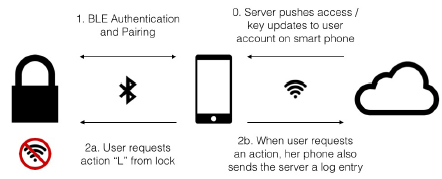
\includegraphics[width=0.7\textwidth]{paperNotes/ho2016_components}
			\caption{Kommunikation zwischen Komponenten des Smart Lock Systems von August}
			\label{fig:gateway}
		\end{figure}

    \subsubsection{Sichereit}
        \paragraph{Rollen und Rechteverteilungen:}
        Relevant: \cite{Ye2017}\cite{Ho2016}
		\begin{itemize}
			\item Rollen: Owner(Grant, Revoke, Lock/Unlock, Admin Features wie Zugriffshistorie), Resident(Lock/Unlock), wiederkehrender Gast (nur Lock/Unlock zu bestimmten Zeitfenstern), temporärer Gast(Lock/Unlock für eine bestimmte Zeit wie 24 Stunden)
			    Die Rolle des Owners wird jenem Gerät vergeben, das sich nach Installation des Smart Locks als erstes mittels \gls{ble} (oder bei einigen Modellen über W-LAN) verbindet.
			    Die Owner-Rolle kann auf diesem Wege nur einmal vergeben werden.
			    Bei Wechsel des Besitzers muss das Smart Lock zurückgesetzt werden.
			    Rollen wieder zu entfernen und somit anderen Nutzers wieder die Rechte zu entziehen, muss Owner sein.
			    Um die Rechte eines Owners bei einem verlorenen oder gestohlenen zu entziehen, wird entweder eine "Lost Phone"-Funktion angeboten oder ein anderer Nutzer mit der Rolle des Owners entzieht dem nicht mehr vorhandenen Gerät die Rolle.
			    Der Owner kann das Schloss auch ohne Internetverbindung öffnen/schließen.
			    Gäste hingegen müssen sich vor der Kommunikation mit dem Schloss gegenüber der dem Server des Herstellers autorisieren lassen.
			\item Permissions: Lock/Unlock, Lock Activity, Guest List, User Invitation (new Users), User Level Control (update User Role), User Permission Control (e.g. set time slots for guests, revoke permissions from users), Schloss kalibrieren und zurücksetzen\cite{Fuller2017}, Activiy Protokoll ansehen\cite{Fuller2017}, Autolocking/-unlocking akivieren/deaktivieren, eigenen Account löschen
		\end{itemize}
		über Secret Keys\cite{Fuller2017}
		\begin{itemize}
		    \item jede Bluetooth-Verbindungssession bekommmt einen eigenen einzigartigen Session-Key (weiter SK genannt), welcher für Owner wie folgt entsteht:
		    \missingfigure{Wie der Session Key für Owner entsteht}
		        \begin{enumerate}
		            \item Das Smartphone sendet zufällige 64 Bit an das Schloss, welche mit dem offline Keys des Smartphones verschlüsselt werden, an das Schloss
		            \item Das Schloss sendet 64 zufällige Bits, die mit dem offline Key des Smartphones verschlüsselt sind, an das Smartphone zurück
		            \item Das Schloss und das Smartphone entschlüsseln die jeweils erhaltene Nachricht und konkatinieren beide Nachrichten zu einer neuen 128-Bit langen Folge, die im weiteren Verlauf als AES-Key zur Verschlüsselung der Session genutzt wird.
		        \end{enumerate}
		        Gäste, welche keinen "offline Key" zugewiesen bekommen, kommunizieren mit dem Webserver:
		        \missingfigure{Wie der Session Key für Gäste entsteht}
		        \begin{enumerate}
		            \item Das Smartphone des Gasts sendet 64 zufällige Bits als Klartext an den Server
		            \item Der Server verschlüsselt diese 64 Bits mit dem Firmware Key und sendet die verschlüsselten Bits als Nachricht an den Gast zurück
		            \item Der Gast leitet den Ciphertext, welcher von dem Server empfangen wurde, an das Schloss weiter.
		            \item Das Schloss sendet 64 Bits mit XY  verschlüsselt an den Gast, welcher diesen Ciphertext an den Server weiterleitet.
		            \item Der Server entschlüsselt die Nachricht und sendet sie als Klartext per SSL an den Gast.
		            \item Das Schloss und der Gast konkatenieren beide 64-Bit langen Folgen zu einem 128-Bit Schlüssel, welcher als Session Key verwendet wird.
		        \end{enumerate}
		    \item SK wird genutzt, um Nachrichten zwischen dem Schloss und dem Smartphone des Nutzers mit AES zu ver- und entschlüsseln
		    \item Voraussetzung: für das Protokoll, welches den Session Key erstellt müssen bereits im Voraus das Schloss und entweder die Webserver des Herstellers oder das Smartphone des Nutzers einen Secret Key teilen.
		    \item in August können insgesamt 256 Schlüssel (von 0-255 nummeriert) gespeichert werden, wobei Nummer 0 besondere Privilegien hat und als "firmware key" angesehen wird (\textrightarrow Hardcoded und somit anfällig, sollte in falsche Hände geraten).
		        Die Webserver des Herstellers, Nutzer mit der Rolle OWNER und das Schloss selbst kennen den Schlüssel.
		        anderen Keys sind "offline Keys", die zur Initialisierung einer Bluetooth-Session verwendet werden, sollte der Nutzer nicht mit dem Internet verbunden sein
		\end{itemize}
		
		
